\documentclass[12pt,twocolumn,letterpaper]{article}

\usepackage{cvpr}
\usepackage{times}
\usepackage{epsfig}
\usepackage{graphicx}
\usepackage{amsmath}
\usepackage{amssymb}
\usepackage[breaklinks=true,bookmarks=false]{hyperref}
\usepackage{gensymb}
\usepackage{subcaption}

\cvprfinalcopy

\def\httilde{\mbox{\tt\raisebox{-.5ex}{\symbol{126}}}}


\setcounter{page}{1}
\begin{document}

\title{Visual Odometry on Smartphone}

\author{Jai Prakash\\
Carnegie Mellon University\\
Master of Science in Computer Vision\\
{\tt\small jprakash@andrew.cmu.edu}
\and
Utkarsh Sinha\\
Carnegie Mellon University\\
Master of Science in Computer Vision\\
{\tt\small usinha@andrew.cmu.edu}
}

\maketitle

\begin{abstract}
In this project, we are trying to localize the camera using visual odometry. The major component of the project is to generate keyframes according to pre-defined heuristics and triangulate the points to create 3D reconstruction of the scene. The intermediate frames can be found using Perspective-n-point algorithm. In addition, we also perform local bundle adjustment over last few frames so that the localization is locally consistent. We also plan to exploit the onboard inertial sensors to get prior for the localization.
\end{abstract}

\section{Introduction}

Augmented reality has been around for years, yet not all problems are solved in that domain. One of the challenges being precise localization of the device in the world. Most of the augmented reality applications on smartphones are based on markers. One good example of marker-based AR is Vuforia. On the other hand, there are standalone devices like Hololens, which has number of sensors to understand the scene and localize the head mounted display in the scene.

In many of the Augmented Reality application, you do not have to understand the scene. Sometimes, just localizing the camera in the world would solve the problem. In this project we focus on localizing the phone using the camera and the inertial sensors.

\section{Background}
\textbf{Visual SLAM vs. Visual Odometry: } The focus in the visual SLAM techniques is both in reconstruting the scene and also localizing the camera in the scene. However, our main focus is just in localization of the camera. For the scope of the project, we focus only to be locally consistent. So, our system might intrduce drift over time.

\begin{figure}
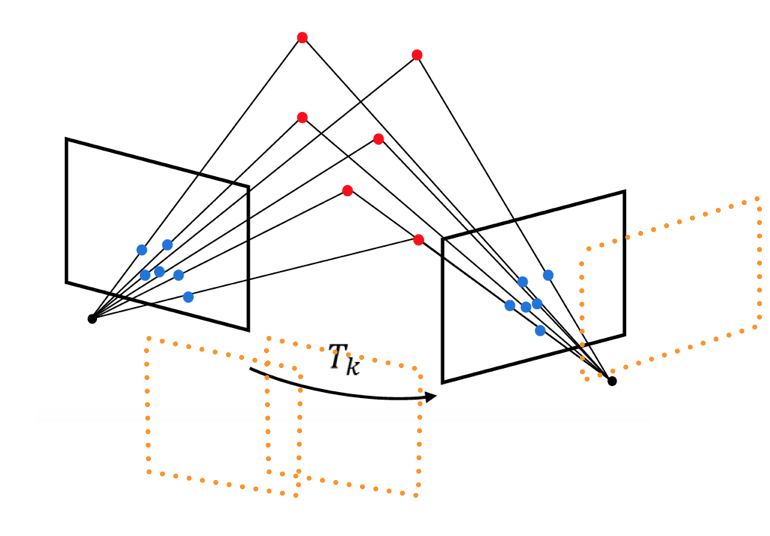
\includegraphics[width=0.5\textwidth]{images/system}
\caption{A visualization of the Visual Odometry system}
\label{fig:system}
\end{figure}

\section{Method}
Our system contains of the following blocks.
\begin{itemize}
\item \textbf{Feature Extraction and matching: } We have experimented with OpenCV KLT features, AKAZE features and ORB features. The KLT features can also be used for tracking the features in the subsequent frames. For AKAZE and ORB features, the correspondences are found using feature matching. The outliers are removed using the epi-polar constraints and finding unique matches i.e. feature from first image matches to a unique feature in second image and vice-versa.

\item \textbf{3D reconstruction: } Using the feature matching, we can triagulate the points. The fundamental matrix gives the relationship between the feature points. We used 8-point algorithm to find the fundamental matrix.

$$ p_2^T F p_1 = 0 $$

The Essential matrix can be found using the equation (assuming the same camera intrinsics in both cameras)
$$ E = K^T F K $$

The essential matrix can be decomposed to rotation and translation component.
$$ E = U\Sigma V^T $$
$$ R = U W U^T $$
$$ t = U \Sigma V^T $$

This gives rise to four possible camera locations. The correct location can be found using the camera configuration in which all the points are in front of both the cameras.

\item \textbf{Camera pose recovery: } Once the scene is reconstructed using the keyframes, the camera pose can be recovered using Perspective-n-point (PnP) algorithms. By knowing the 3D points from the reconstruction, and its corresponding feature location in any image the camera pose can be recovered using PnP.

\item \textbf{Bundle Adjustment: } In visual odometry, the current camera pose is
obtained by adding the last observed motion to the
current detection change. This leads to a super-
linear increase in pose error over time. In this
section, we look at the techniques we intend to
use to correct this pose drift
One solution is to use bundle adjustment to impose geometrical constraints over multiple
frames. The computational cost increases with
the cube of the number of frames used for com-
putation. Thus, we limit the number of frames
to a small window from the previously captured
frames.

\end{itemize}

\begin{figure}
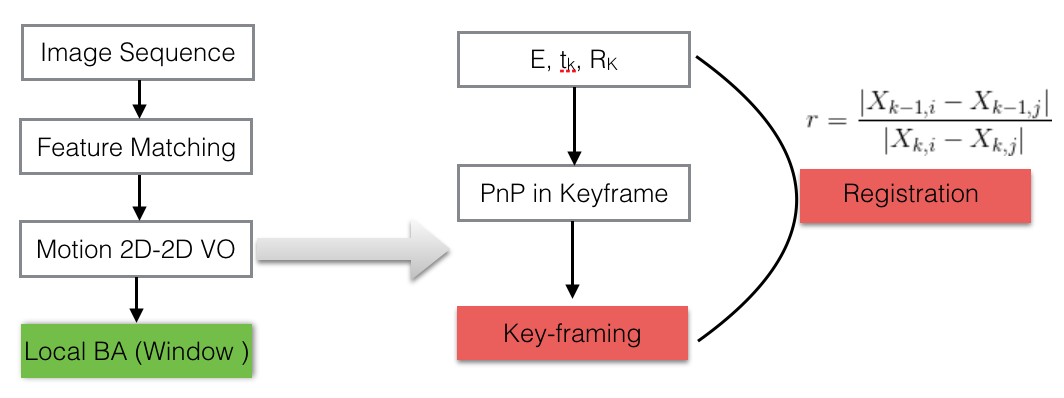
\includegraphics[width=0.5\textwidth]{images/block}
\caption{Block diagram of the system. The red blocks are implemented as a part of Geometry based vision project. For this project we are focusing on implementation of local bundle adjustment shown in green}
\label{fig:block}
\end{figure}


\section{Results}
So far, we have been working with the datasets available online. The results are illustrated on the Middlebury Temple dataset \cite{middlebury}. We first find the feature correspondences and then remove the outliers using Epipolar constraints. The outliers can be found by using a threshold on distance from epi-polar line and along the epipolar line.

We are able to recosntruct the temple structure using the two keyframes (handpicked for now). The results are shown in figure \ref{fig:reconstruction}. Once the reconstruction is done, we are able to recover the camera poses using PnP algorithm as illustrated in the figure \ref{fig:pose}. We are using OpenCV for feature matching and visualization.


\begin{figure}
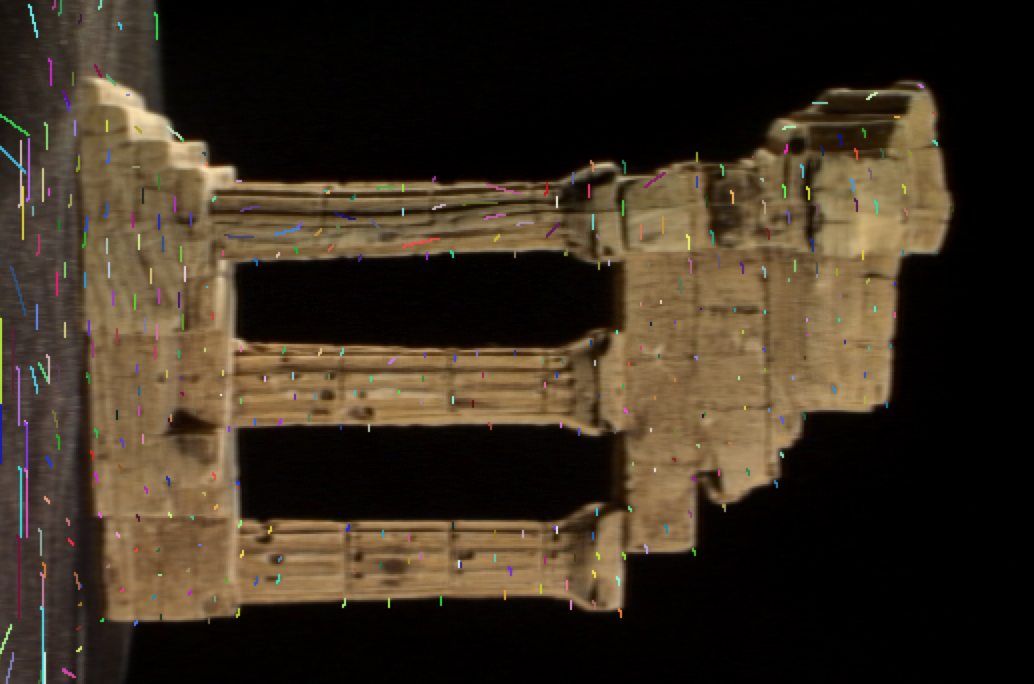
\includegraphics[width=0.5\textwidth]{images/temple_correspondence}
\caption{Temple correspondence using KLT features}
\label{fig:correspondence}
\end{figure}

\begin{figure}
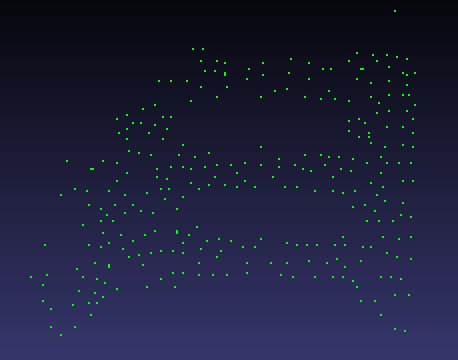
\includegraphics[width=0.5\textwidth]{images/temple1}
\caption{Temple reconstruction using keyframes}
\label{fig:reconstruction}
\end{figure}

\begin{figure}
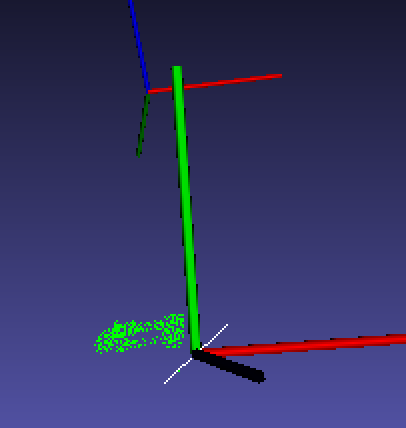
\includegraphics[width=0.5\textwidth]{images/camera_pose}
\caption{Recovered camera poses using PnP. The 3D points are obtained using keyframes. The camera pose is found using its corresponding feature in the image}
\label{fig:pose}
\end{figure}


\section{Future Work}
\begin{itemize}
\item Evaluation of various features. 
\item Integration of inertial sensor in the pipeline
\item Integration of Google Ceres-solver for bundle adjustment.
\end{itemize}

    
{\small{
\begin{thebibliography}{15}

\bibitem{Szeliski}
Szeliski, Richard. \textit{Computer Vision: Algorithms and Applications}. 1st ed. London: Springer-Verlag, 2010. Print.

\bibitem{middlebury} 
Temple dataset \url{http://vision.middlebury.edu/mview/data/}

\endgroup
\end{document}
